\documentclass[12pt]{article}
\usepackage[utf8]{inputenc}
\usepackage[usenames]{color}
\usepackage[margin=1in]{geometry} 
\usepackage{amsmath,amsthm,amssymb,graphicx,mathtools,tikz,hyperref, pgfplots, listings, pdfpages}
\usetikzlibrary{positioning}
\newcommand{\n}{\mathbb{N}}
\newcommand{\z}{\mathbb{Z}}
\newcommand{\q}{\mathbb{Q}}
\newcommand{\cx}{\mathbb{C}}
\newcommand{\real}{\mathbb{R}}
\newcommand{\field}{\mathbb{F}}
\newcommand{\ita}[1]{\textit{#1}}
\newcommand{\com}[2]{#1\backslash#2}
\newcommand{\oneton}{\{1,2,3,...,n\}}
\newcommand\idea[1]{\begin{gather*}#1\end{gather*}}
\newcommand\ef{\ita{f} }
\newcommand\eff{\ita{f}}
\newcommand\proofs[1]{\begin{proof}#1\end{proof}}
\newcommand\inv[1]{#1^{-1}}
\newcommand\setb[1]{\{#1\}}
\newcommand\en{\ita{n }}
\newcommand{\vbrack}[1]{\langle #1\rangle}


\newenvironment{theorem}[2][Teorema]{\begin{trivlist}
\item[\hskip \labelsep {\bfseries #1}\hskip \labelsep {\bfseries #2.}]}{\end{trivlist}}
\newenvironment{lemma}[2][Lema]{\begin{trivlist}
\item[\hskip \labelsep {\bfseries #1}\hskip \labelsep {\bfseries #2.}]}{\end{trivlist}}
\newenvironment{exercise}[2][Ejercicio]{\begin{trivlist}
\item[\hskip \labelsep {\bfseries #1}\hskip \labelsep {\bfseries #2.}]}{\end{trivlist}}
\newenvironment{reflection}[2][Reflexión]{\begin{trivlist}
\item[\hskip \labelsep {\bfseries #1}\hskip \labelsep {\bfseries #2.}]}{\end{trivlist}}
\newenvironment{proposition}[2][Proposición]{\begin{trivlist}
\item[\hskip \labelsep {\bfseries #1}\hskip \labelsep {\bfseries #2.}]}{\end{trivlist}}
\newenvironment{corollary}[2][Corolario]{\begin{trivlist}
\item[\hskip \labelsep {\bfseries #1}\hskip \labelsep {\bfseries #2.}]}{\end{trivlist}}
 \hypersetup{
 colorlinks,
 linkcolor=blue
 }

\renewcommand{\ttdefault}{pcr}
\lstdefinestyle{C}{language=C,
    basicstyle=\ttfamily,
    keywordstyle=\bfseries,
    showstringspaces=false,
    morekeywords={include, printf},
	keepspaces=true,numbers=left,xleftmargin=2em,frame=shadowbox,framexleftmargin=0 em, rulesepcolor = \color{black}
}
\lstdefinestyle{linuxterminal}{language=bash,
    basicstyle=\ttfamily,
    keywordstyle=\bfseries,
    showstringspaces=false,
    morekeywords={include, printf},
	keepspaces=true,
	frame=TLRB
}


\begin{document}
	\date{18-04-2018}
	
	
	\title{\textbf{\textcolor{red}{INFORME PROYECTO FINAL}}}
	\author{Alejandro Santorum Varela - alejandro.santorum@estudiante.uam.es\\David Cabornero Pascual - david.cabornero@estudiante.uam.es\\Pr. SOPER - Pareja 7\\Universidad Autónoma de Madrid}
	\maketitle
	
	\tableofcontents
	
	\newpage
	
\section{Introducción}
Llegamos a la última entrega de las prácticas de Sistemas Operativos. Esta vez es "un único ejercicio", que engloba todo lo visto y estudiado hasta el momento.\\

El proyecto final consiste en un simulador de una carrera de caballos que funciona de forma distribuida. Varios son los procesos que deberán de coordinarse para desarrollar la carrera, las apuestas y enseñar toda esta información por pantalla.\\

A continuación se comenta la implementación de cada proceso y el por qué se ha optado tal diseño.\\

\section{Esbozo inicial}
Se muestra a continuación un esquema inicial de la generación de los procesos, que serán descritos más adelante con más profundidad.
\begin{center}
	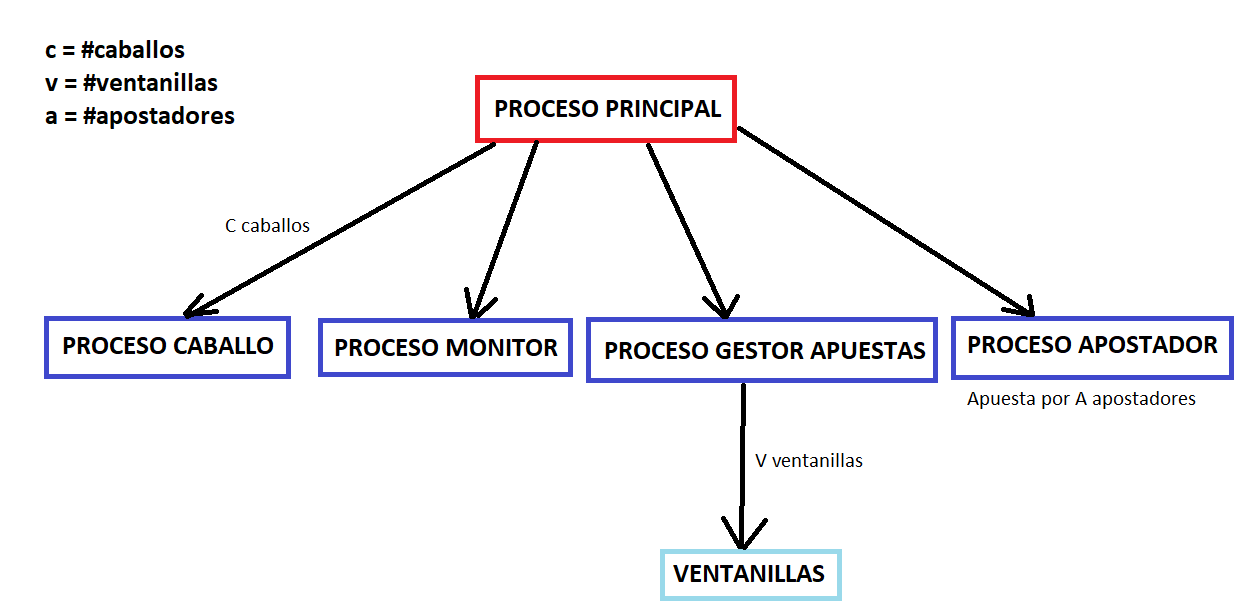
\includegraphics[scale=1]{gerarquia.png}
\end{center}

\section{Proceso apostador}
Es el proceso encargado de simular la acción de una persona que desea apostar por un caballo.\\

En la documentación del proyecto se describe a este proceso diciendo que tiene que realizar una apuesta por segundo, pero creemos que esto es un error de traducción de la práctica el año pasado pues, si solo tenemos un único proceso apostador que debe realizar apuestas por todos los apostadores y tenemos un tiempo de apuestas de 30 segundos, \textbf{entonces si hay 100 apostadores 70 de ellos no llegarían a apostar}.\\

El cambio que se ha tomado es el más lógico: el proceso apostador escogerá un apostador aleatorio, un caballo aleatorio y una cantidad de dinero aleatoria y esa será la nueva apuesta. Toda esta información será enviada por una cola de mensajes al proceso manejador de apuestas, que procesará dicha información.\\

Comentar que el dinero de los apostadores (valor introducido como parámetro de entrada al programa) es la cantidad máxima apostable. Es decir, en cada apuesta tendrá una cantidad de dinero apostada variable entre 0 y este valor introducido para todos los apostadores. Esto es así porque si decidimos que este parámetro es el dinero disponible para los apostadores, en menos de un segundo habrán consumido totalmente su dinero debido a la velocidad normal de un programa informático, y por lo tanto las cotizaciones de los caballos que se deben mostrar por pantalla en esos 30 segundos \textbf{no variarán}.\\

En resumen, el proceso apostador escoge un apostador aleatorio, un caballo aleatorio, y una cantidad aleatoria dentro de unos límites establecidos y envía todo esto al proceso gestor de apuestas para ser procesado.\\

\section{Proceso gestor de apuestas}
Este proceso tiene una vida de 30 segundos, el tiempo disponible para las apuestas.\\

Su misión comienza incializando todas las apuestas. Estas apuestas están almacenadas en una zona de memoria compartida para que tanto el proceso gestor de apuestas como el proceso monitor puedan acceder a ellas en tiempo real. Por esta razón, necesitamos un semáforo protegiendo dicha zona de memoria para que no puedan acceder ambos a la vez.\\

Las apuestas son iniciadas según se indica en la documentación: total de dinero apostado a cada caballo = 1, cotización de cada caballo igual al dinero apostado a todos los caballos \textbf{hasta ese momento} partido del dinero apostado al caballo \textbf{hasta ese momento}. Por último consideramos que el dinero a pagar a cada apostador es incialmente cero.\\

Con esta forma de inicializar las apuestas, las cotizaciones de los caballos quedarían de la siguiente forma:\\
· Cotización caballo 1 $= 1/1 = 1$.\\
· Cotización caballo 2 $= 2/1 = 1$.\\
···\\
· Cotización caballo n $= n/1 = n$.\\

Después de inicializar las apuestas, este proceso deberá crear tantos hilos (ventanillas de apuestas) como se haya introducido por línea de comandos. Estos hilos serán los que recojan los mensajes de apuestas de la cola de mensajes procedientes del proceso apostador y actualizarán las cotizaciones de cada caballo. Además, imprimirán en un fichero ("apuestas.txt") todas las apuestas procesadas para poder calcular los beneficios de cada apostador al final de la carrera.\\

Las cotizaciones de los caballos serán actualizadas de la siguiente manera: cotización caballo = total dinero apostado a todos los caballos / total dinero apostado al caballo. Recordemos que el caballo n tiene una cotización inicial de n, lo que es bastante. Pueden dispararse los beneficios y/o las cotizaciones si un apostador apuesta una gran cantidad a este caballo. Esto no sería raro debido a que tanto el caballo como la cantidad son escogidas aleatoriamente.\\

Una vez que la carrera comienza, las apuestas finalizan. En la cola de mensajes de apuestas habrá una cantidad de apuestas sin procesar, pero las ventanillas cerrarán nada más comenzar la carrera. Esta sincronización se realiza por medio de señales entre el proceso principal, el monitor, y el gestor de apuestas.\\

\section{Proceso monitor}
El proceso monitor es el encargado de presentar por pantalla la información relevante. Tiene tres fases claramente diferenciables.\\

La primera es la que muestra por pantalla las cotizaciones actualizadas de cada caballo antes de que comience la carrera. Las cotizaciones son actualizadas cada segundo, entonces este proceso imprimirá 30 veces las cotizaciones de los caballos. No obstante, las cotizaciones habrán podido variar en ese segundo de margen entre impresión e impresión, por lo que no quiere decir que todas las apuestas se hayan con esas cotizaciones.\\

Como se ha comentado, las cotizaciones son almacenadas en una zona de memoria compartida, por lo que cada vez que el proceso monitor muestra por pantalla esta información, deberá de ayudarse de un semáforo para no alterar los resultados.\\

La segunda fase muestra el estado de la carrera en cada instante. El estado de la carrera, igual que el estado de las apuestas, es almacenado en otra zona de memoria compartida (protegida por otro semáforo). Se utilizan preferiblemente zonas de memoria compartida porque son más sencillas (y el código es más claro) que las colas de mensajes. Solo hay que tener cuidado con la correcta colocación de los semáforos.\\

En esta fase, se mostrará el identificador de caballo, su posición y su casilla actual. Esta información será actualizada por pantalla cada vez que \textbf{todos} los caballos hayan tirado los dados y hayan comunicado el resultado al proceso principal para actualizar su posición.\\

Finalmente, la última etapa de este proceso es cuando la carrera ya ha finalizado. Imprimirá la clasificación final de la carrera: identificador de caballo, su posición final y su casilla final. Además, mostrará los 10 mejores apostadores, es decir, los apostadores con más beneficios. Si escogemos un número de apostadores igual o parecido a 10, algunos de ellos aparecerán con beneficios negativos, debido a que no les han ido muy bien las apuestas. Todos los datos finales de los apostadores serán almacenados en un fichero de texto llamado "resultados\_apostadores.txt".\\

\section{Proceso caballo}
En la carrera, cada caballo será un proceso distinto, cada uno con un ID o identificador diferente.\\

Durante el tiempo de apuestas permanecen todos a la espera, como si del semáforo verde en una carrera de F1 se tratase. Cuando el tiempo de apuestas finaliza, el proceso principal "pone el semaforo en verde", lo que viene a ser enviarle una señal a todos los caballos para comunicarles que pueden comenzar la carrera.\\

Los caballos utilizan la memoria compartida de control de carrera para actualizar \textbf{su} última tirada. Cuando la han actualizado actualizan una variable compartida llamada \emph{horses\_done} que se encarga de impedir que un caballo tire dos veces mientras uno aun no haya tirado debido a condiciones de carrera. Una vez incrementada dicha variable hasta el número total de caballos, lo que quiere decir que todos han actualizado su última tirada, despiertan al proceso principal para que recalcule la clasificación.\\

Con la actualización de la clasificación, ya se sabe que caballos tienen derecho a tiradas remontadoras y ganadoras, lo cual también es comunicado a los caballos.\\

Una vez que un caballo llegue a meta, el proceso principal será el encargado de terminar con la ejecución de todos los procesos caballos mediante la señal SIGNINT.\\

\section{Proceso principal}
Finalmente, vamos a comentar la implementación del proceso principal.\\

Ya se conoce algunas de sus funciones por haber sido comentadas ligeramente en la descripción del resto de procesos, pero aquí las subrayaremos.\\

Para empezar, como es lógico el proceso principal comprobará que todos los parámetros de entrada son correctos. Si esto tiene éxito, preparará todas las vías de intercomunicación entre todos los procesos e hilos: una cola de mensajes, dos zonas de memoria compartida, tres semáforos (que protegen dos zonas de memoria y un fichero accedido por varios procesos/hilos).\\

Comentar que el proceso principal no se comunica con los caballos mediante tuberías por unas cuantas razones. En primer lugar no son "solo" el proceso principal y los caballos los únicos que tienen que saber la clasificación actualizada en todo momento durante la carrera, sino que el proceso monitor también la necesita. En la documentación aparece que se comuniquen los caballos con los proceso principal con tuberías y estos con el proceso monitor mediante colas de mensajes, pero es realmente ineficiente, tanto para el coste computacional(memoria requerida y tiempo de ejecución) como coste "mental" para nosotros a la hora de coordinar todo esto. Se necesitarían $2n$ tuberías, siendo $n$ el número de caballos, para comunicar el proceso principal con los caballos y otras $2n$ tuberías para comunicar los caballos de nuevo con el proceso principal, ya que no son bidireccionales.\\

Por todo esto, hemos optado por utilizar una zona de memoria compartida protegida por un semáforo. Esto requiere una menor cantidad de memoria y un tiempo de ejecución menor.\\

Después de crear todos estos mecanismos de comunicación, crea todos los procesos necesarios para la simulación y ejecuta su función característica.\\

Una vez que comience la carrera tendrá la importante tarea de actualizar las posiciones de cada caballo con sus tiradas y comunicarles a los mismos su estado para poder realizar las diferentes tiradas. El proceso monitor actualizará dicha clasificación en un intervalo entre 2 y 3 segundos para poder analizar cada momento de la carrera con detenimiento.\\

Una vez terminada la carrera, el proceso principal indicará mediante una señal a los caballos de su finalización, y al proceso monitor de que puede proceder a mostrar por pantalla los resultados finales de la carrera y de las apuestas.\\

Una vez que el proceso monitor finalice, proceso principal eliminará todas las zonas de memorias compartidas, las colas de mensajes, y la memoria reserrvada para finalizar exitosamente la simulación.\\

\newpage
\section{Diagrama de flujo}
Se muestra a continuación el diagrama de flujo que posiblemente ayude a comprender el order de actuación de todos los procesos.
\begin{center}
	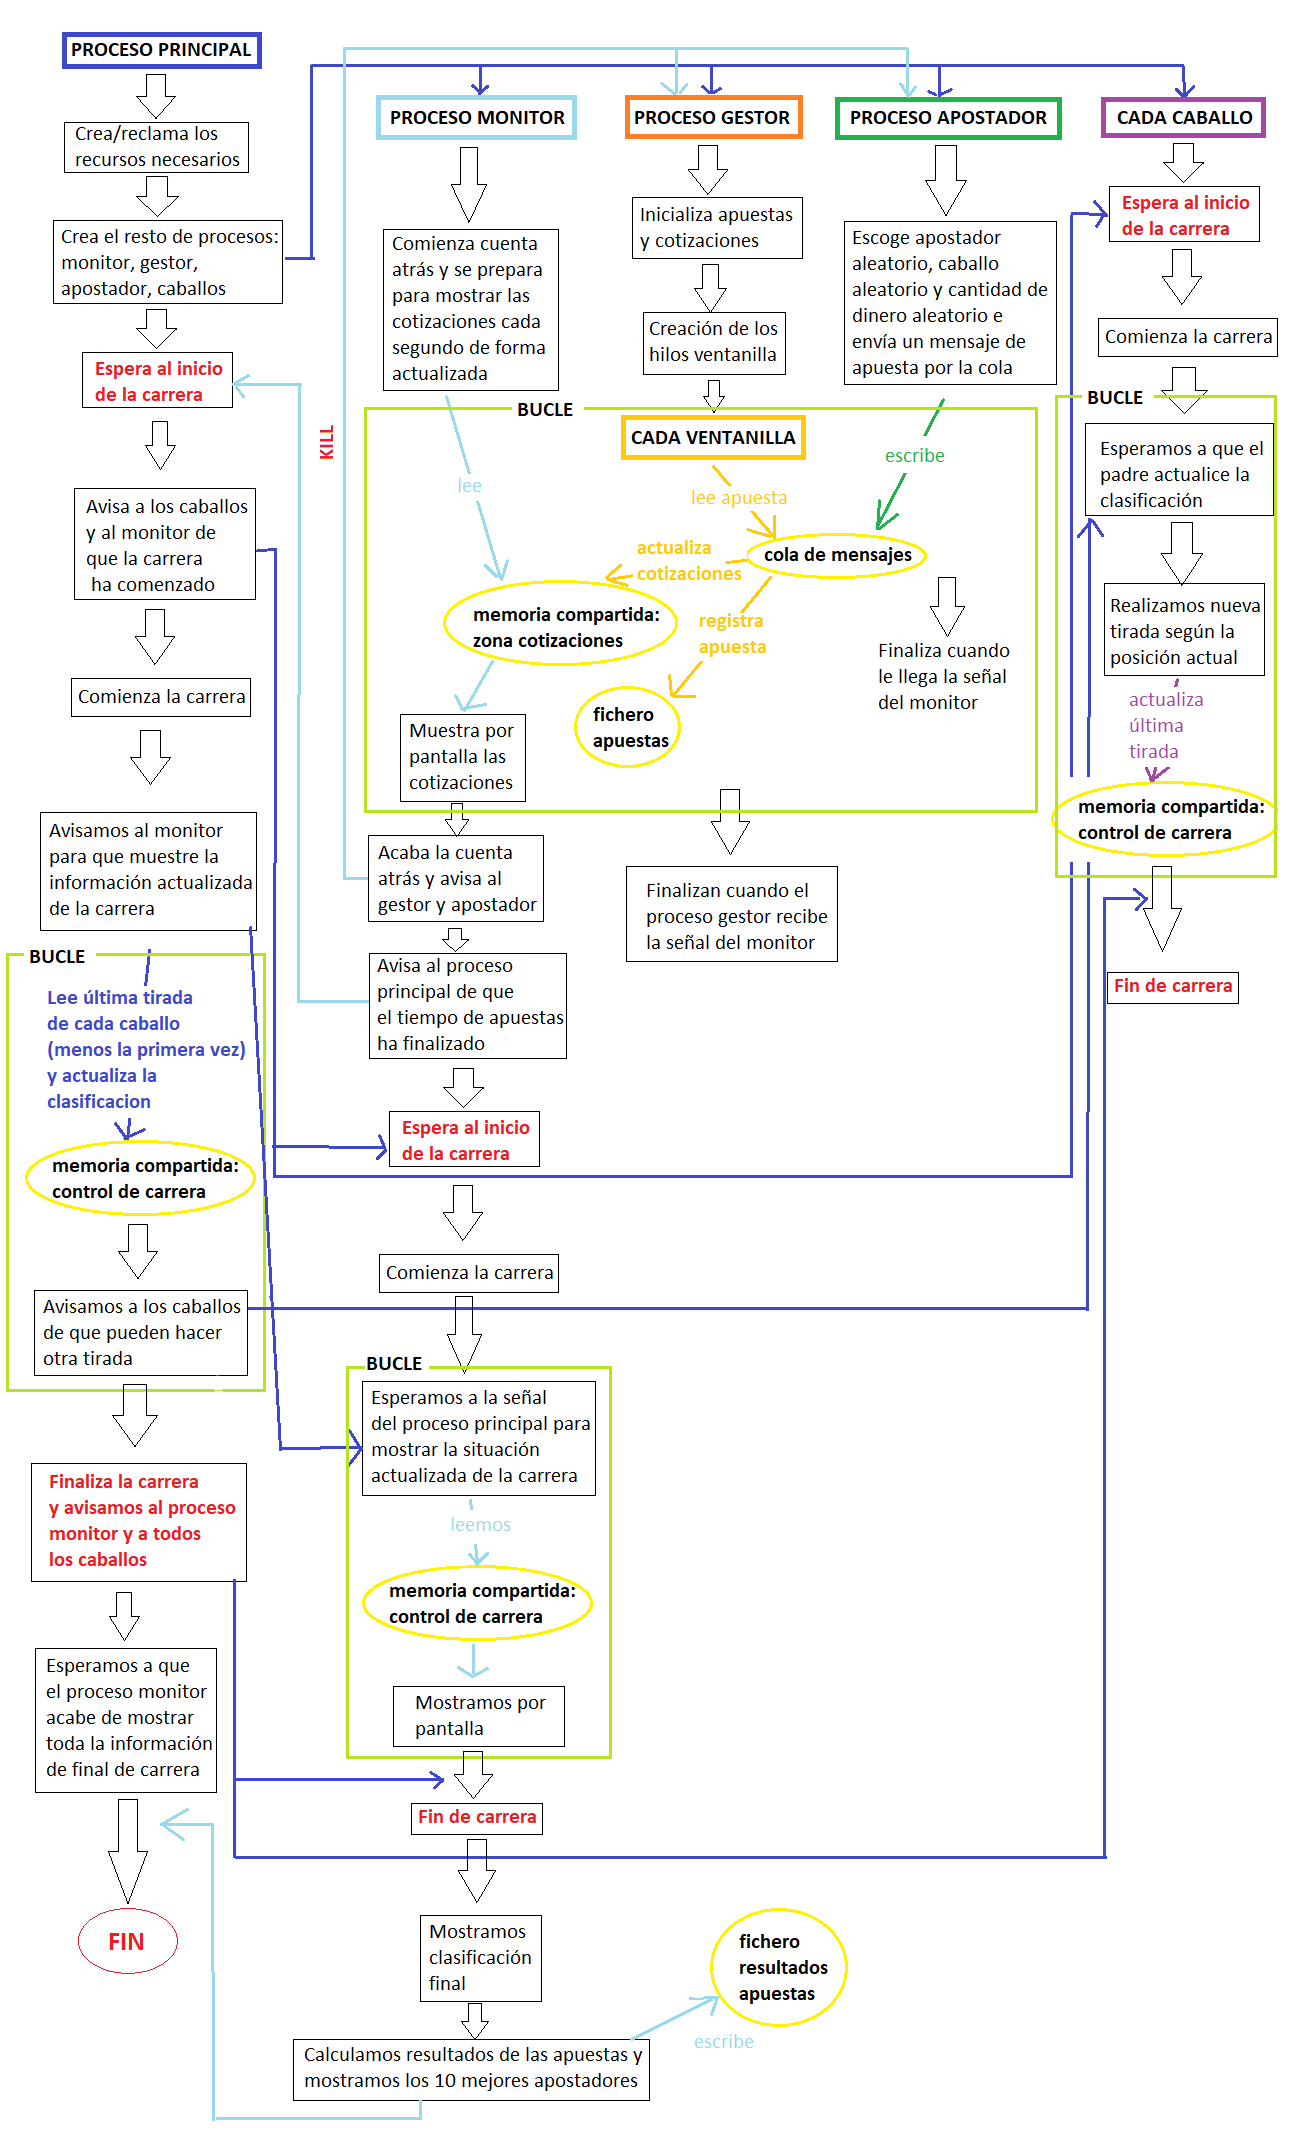
\includegraphics[scale=0.73]{diagrama_flujo.png}
\end{center}

\section{Salida - Output}
Se muestran a continuación un par de imágenes de una ejecución aleatoria del programa. Los parámetros utilizados son 8 caballos, longitud de la carrera igual a 20, 10 apostadores, 8 ventanillas y dinero máximo apostable igual a 100.\\

Informe de memoria de \emph{valgrind} del proceso principal:
\begin{center}
	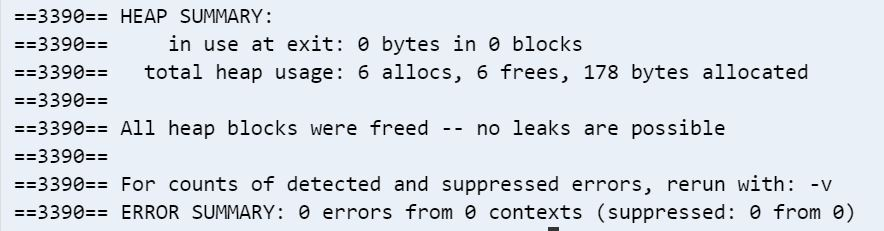
\includegraphics[scale=0.8]{valgrind.JPG}
\end{center}

Salida final de carrera y mejores apostadores:
\begin{center}
	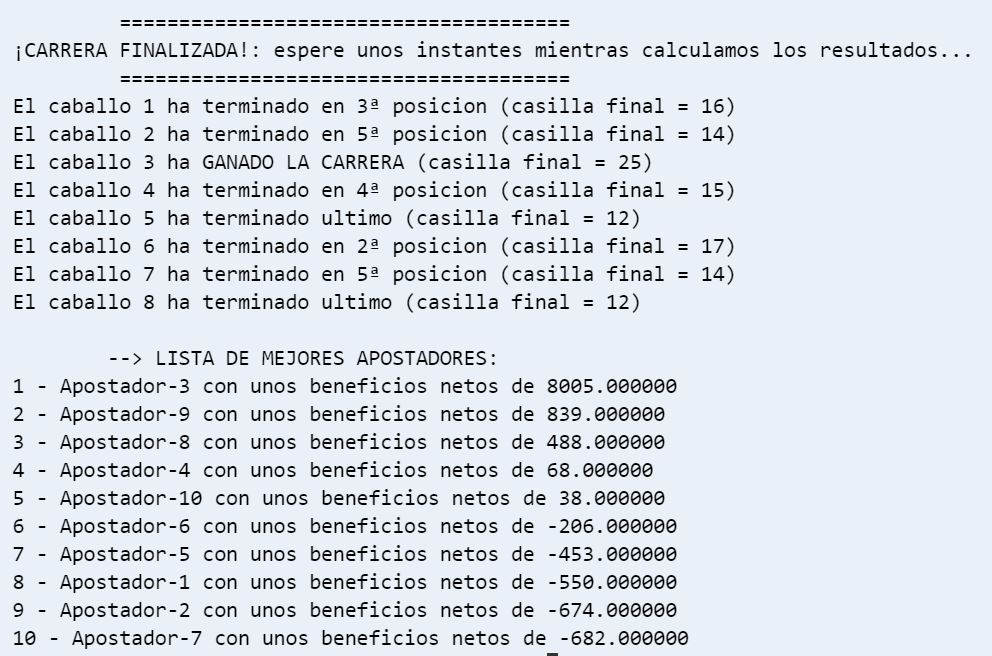
\includegraphics[scale=0.8]{resultados_carrera.JPG}
\end{center}

\section{Conclusión}
Ha sido la práctica más bonita y divertida de todas, principalmente porque los conceptos ya estaban medio adoptados, por lo que nos limitamos a programar y no tanto a "estudiar" el \emph{man} y las funcionalidades de cada función.\\

Por otro lado, el proyecto ha servido para sustentar conceptos ya aprendidos y aclarar su funcionalidad.\\

Como toda práctica, el programa \textbf{nunca} se ejecuta a la primera y hemos tenido que lidiar con los posibles fallos de código, coordinación de procesos, posibles interbloqueos, keys de sistema no aptas para la creación de semáforos, zonas de memoria compartida, etc. Pero hemos podido sobrevivir una vez más y sacar adelante otra tarea.\\

Un placer haber asistido a esta asignatura y en especial a la clase de prácticas, mucho más interativa que la teórica.
\end{document}